\subsection{Blobs}\label{sec:blobs}
En blob er en sammenhængende region af pixels, der enten er betydeligt lysere eller mørkere end dens omgivelser, altså strukturer, der står i kontrast til deres baggrund. En blob kan derfor udvælges som værende et lokalt ekstrema i billedet. Blobbens omfang strækker sig til punktet hvor den møder en anden blob. Dette kan intuitivt beskrives for lyse-blobs på en mørk baggrund, ved at betragte billedets funktion som et landskab dækket af vand. Sænkes vandet, vil toppe af billede funktionen gradvist dukke op. Sænkes vandet yderligere vil to toppe forbindes, 'dalen' hvor de to toppe mødes vil afgrænse deres omfang. Et sådant punkt hedder et saddle-point, som set i figur \ref{fig:lindblob} og definere et punkt der har geometriske krumninger i hver sin retning.
\begin{figure}[H]
    \centering
    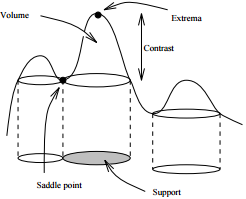
\includegraphics[width=0.35\textwidth]{fig/11.png}
    \vspace{-0.5em}   
    \begin{center}
    \caption{\textcolor{gray}{\footnotesize \textit{
    En blob visualiseret i 2-d, udefra Lindenberg's definition \cite{blob}}}}
    \label{fig:lindblob}
     \end{center}
  \end{figure}
       \vspace{-2.7em}
\noindent
En blob kan udvælges ved at identificere den geometriske struktur i om omkring et punkt. De to principielle krumninger i et punkt angiver, hvor meget overfladen bøjer i de forskellige retninger. Da et ekstrema angiver en blob, vil de principielle krumninger for punktet være ens. For et punkt placeret på et maksima vil de principielle krumninger være konkave (nedadgående) og for et punkt placeret på et minima vil de principielle krumninger være konvekse (opadgående). For et saddle-point vil den ene krumning være konkav og den anden konveks. \\ 
Om et punkt i billedet er placeret på et maksima, minima eller saddle-point, kan determineres ved en 'to variabel, anden-afledte-test'. Dette udføres ved at opstille en matrice, der indeholder, for et givent punkt, dens dobbeltafledte i x, y og xy retningen, også kaldet Hessian matricen $\mathcal{H}$.
\begin{equation}
\mathcal{H} = 
 \begin{bmatrix}
 	L_{xx} & L_{xy} \\
 	L_{xy} & L_{yy}
 \end{bmatrix}
 \label{hessianmatrixblob}
\end{equation}
hvor den andenafledte i x retningen defineres ved:
\begin{equation}
L_{xx}(x, \sigma) = (\frac{\partial^2 }{\partial x^2 } G(x,y,\sigma)) * I
\label{lxx}
\end{equation}
Egenvektorerne for $\mathcal{H}$ beskriver retningerne for de principielle krumninger af et punkt, hvor egenværdierne beskriver størrelserne af disse krumninger. Den geometriske struktur kan derved defineres ud fra Hessian matricens egenværdier $\lambda_1 \& \lambda_2$:
\begin{equation}
\begin{split}
indikator = 
\begin{cases}
\text{Minima} & \text{hvis } \lambda_1, \lambda_2 > 0, \\
\text{Maksima}& \text{hvis } \lambda_1, \lambda_2 < 0,  \\
\text{Saddle-Point} & \text{hvis } \lambda_1 \cdot \lambda_2 < 0.
\end{cases}
\end{split}
\label{maxsurp}
\end{equation}
En måde at estimere egenværdiernes fortegn, er ved at tage determinanten af hessian matricen:
\begin{equation}
\textbf{det}\mathcal{H} = L_{xx}L_{yy}-L_{xy}^2
\label{detofhessian}
\end{equation}
Da $\bold{det}(\mathcal{H})=\lambda_1 \cdot \lambda_2$ vil fortegnet af determinanten angive om et punkt er et ekstrema eller et saddle-point:
\begin{equation}
\begin{split}
\text{indikator} = 
\begin{cases}
\text{Ekstrema}& \text{hvis } \bold{det}(\mathcal{H}) > 0,  \\
\text{Saddle-Point} & \text{hvis } \bold{det}(\mathcal{H}) < 0.
\end{cases}
\end{split}
\label{detman}
\end{equation}
Figur \ref{fig:makssad} illustrere, hvordan determinanten af hessian matricen approksimere den geometriske struktur i billedet med et andengradspolynomium. Figuren viser approksimeringen, med et punkt lokaliseret på et maksima og et saddle-point.
\begin{figure}[H]
    \centering
    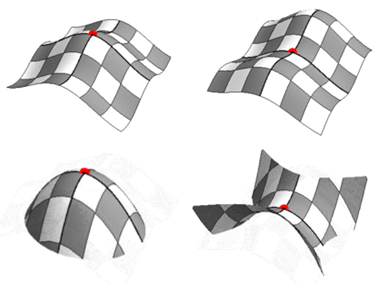
\includegraphics[width=0.50\textwidth]{fig/41.png}
    \vspace{-0.5em}
    \begin{center}
    \caption{\textcolor{gray}{\footnotesize \textit{
d   }}}
    \label{fig:makssad}
     \end{center}
  \end{figure}
       \vspace{-2.7em}
\noindent
En anden metode at detektere blobs er ved Laplace operatoren, som giver et stærkt respons i centeret af en blob. Laplace operatoren kan defineres ved:
$$
\nabla^2L(x,y) = (L_{xx}+L_{yy})
$$
Laplace operatoren svarer til sporret af Hessian matricen. Da $\bold{Tr}(\mathcal{H}) = \lambda_1 + \lambda_2$, vil responset fra laplace operatoren $\nabla^2L$, fortælle noget om egenværdierne og derved den principielle krumning omkring punktet. Et negativt respons, vil angive et maksima da egenværdierne begge vil være negative. Et positivt respons vil angive et minima da egenværdierne begge vil være positive.
\begin{equation}
\begin{split}
\text{indikator} = 
\begin{cases}
\text{Maksima}& \text{hvis } \nabla^2L < 0,  \\
\text{Minima} & \text{hvis } \nabla^2L > 0.
\end{cases}
\end{split}
\label{detman}
\end{equation}
Anvendes Laplace operatoren på Gaussfunktionen (ligning \eqref{2dgaussian}), kan resultatet diskretiseres og anvendes som en kerne, der kan foldes med et billede for identifere forekomster af blobs.
\begin{equation}
LoG= \nabla^2 G
\label{lap}
\end{equation}
Ved oprettelse af et skalarum udglattes regioner i billedet, til grovere strukturer. Bedes man udpege strukturer der gengår på tværs af skalaer (bestående af grove strukturer) vil det være naturligt at udvælge lyse/mørke pletter (blobs), da de vil korrelere nogenlunde i placering og struktur. Dette skyldes blobbens sammenhængende struktur, der gør dem stabile over et større skalainterval. Som nævnt vil et stort respons (postivit eller negativt) til Laplace operatoren definere en blob. Dette er dog kun tilfældet, hvis størrelsen af Laplace filteret matcher størrelsen af blobben. Igen er en aksiomatisk tilgang at gradvist forøge størrelsen af laplace operatoren for det eksisterende skalarum, og udvælge skalaen, hvor der afgives et maksimalt respons. Figur \ref{fig:laprespons} illustrere et respons på en blob af konstant størrelse, udsat for forskellige størrelser af LOG. <genformuler>
\begin{figure}[H]
    \centering
    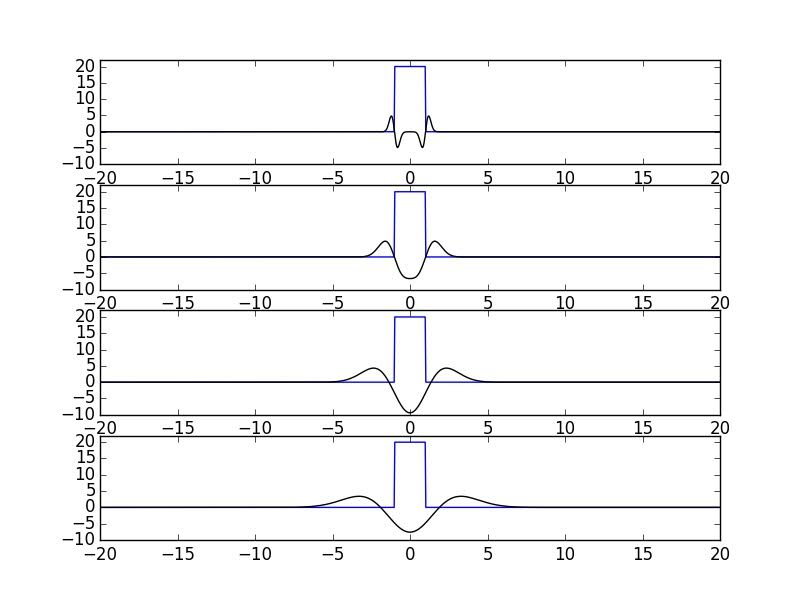
\includegraphics[width=0.80\textwidth]{fig/42.jpg}
    \vspace{-0.5em}
    \begin{center}
    \caption{\textcolor{gray}{\footnotesize \textit{
d   }}}
    \label{fig:laprespons}
     \end{center}
  \end{figure}
       \vspace{-2.7em}
\noindent
En egenskab ved skalapræsentationen er at amplituden af de rumlige afledte vil falde. Dette er, som nævnt i sektion <scale>, grundet
 at maksima over skala ikke kan forøges og minima ikke formindskes. Amplituden af ekstremaer vil derfor altid formindskes over skala <citelindphd>. Dette resultere i at svaret for et filter, som LOG, vil forfalde over skala, <når skalaparametren øges>. For at vedligeholde et konsistent respons over skalaen skal responset normaliseres ift. skala. Da LOG er den andenafledte af et Gauss filter, multipliceres responset med $\sigma^2$. En skalanormaliseret Laplacian of Gauss, kan derfor opskrives som:
$$\nabla^2_{norm}G = \sigma^2(L_{xx}+L_{yy})$$